\documentclass{beamer}
\usetheme{Madrid}
\usepackage{array}
\usepackage{tikz}
\usepackage{multicol}
\usepackage{mathtools}
\title[CST 301 M5]{FORMAL LANGUAGES AND AUTOMATA THEORY}
\subtitle{Module 5}
\author{Rijin IK}
\institute[VJEC]{Assistant Professor\\Department of Computer Science and Engineering\\Vimal Jyothi Engineering College\\Chemperi}
\begin{document}
	\begin{frame}
		\titlepage
	\end{frame}
   \begin{frame}{Outline}
   \tableofcontents
   \end{frame}
\section{Course Outcomes}
\begin{frame}{Course Outcomes}
\textbf{After the completion of the course the student will be able to}
\begin{enumerate}
	\item Classify a given formal language into Regular, Context-Free, Context
	Sensitive, Recursive or Recursively Enumerable. [Cognitive knowledge
	level: Understand]
	\item Explain a formal representation of a given regular language as a finite state
	automaton, regular grammar, regular expression and Myhill-Nerode
	relation. [Cognitive knowledge level: Understand]
	\item Design a Pushdown Automaton and a Context-Free Grammar for a given
	context-free language. [Cognitive knowledge level : Apply]
	\item Design Turing machines as language acceptors or transducers. [Cognitive
	knowledge level: Apply]
	\item Explain the notion of decidability. [Cognitive knowledge level:
	Understand]
\end{enumerate}
\end{frame}
\section{Context Sensitive Languages}
\begin{frame}{Context Sensitive Grammar}
\textbf{Context Sensitive Languages}
\begin{itemize}
	\item A context sensitive grammar (CSG) is an unrestricted grammar in which all the productions are of the form
	$$\alpha \rightarrow \beta$$ Where $\alpha, \beta \in (V\cup T)^+\  and\  |\alpha |\leq | \beta |.$
	\begin{itemize}
		\item Where $\alpha, \beta $\ are strings of terminals and non- terminals.
	\end{itemize}
\item A context sensitive grammar can never generate a language containing the empty string $\epsilon$; $x\rightarrow \epsilon$ not allowed.
\item A context sensitive grammar (CSG) can be converted into normal form where all productions are of the form,
$$\alpha A\beta \rightarrow \alpha \gamma \beta\  where\ \gamma \neq \epsilon$$
\item During derivation non-terminal $A$ will be replaced by $\gamma$ only when it is present in context of $\alpha$ and $\beta$
\item This definition shows clearly one aspect of this type of grammar; it is
\textbf{noncontracting}, in the sense that the length of successive sentential
forms can never decrease.
\end{itemize}
\end{frame}
\begin{frame}{Context Sensitive Languages}
	\textbf{Formal definition of Context Sensitive Grammar}
	\begin{itemize}
		\item A context sensitive grammar $G = (V, T, P, S)$ , where
		\begin{itemize}
			\item V is a set of nonterminal symbols
			\item T is a set of terminal symbols
			\item S is the start symbol, and
			\item P is a set of production rules, of the form $\alpha A \beta \rightarrow \alpha \gamma \beta$ where $A$ in V, $\alpha$, $\beta \in (V\cup T)^*$and $\gamma \in  (V \cup T)^+$
		\end{itemize}
	\end{itemize}
	$^*$The production $S \rightarrow \epsilon$ is also allowed if S is the start symbol and it does not appear on the right side of any production.
\end{frame}
\begin{frame}{Context Sensitive Languages}
	\textbf{Context Sensitive Language}
	\begin{itemize}
		\item A language L is said to be context-sensitive if there exists a
		context-sensitive grammar G, such that $L = L(G).$
		\item If G is a Context Sensitive Grammar then,
		$$L(G) = \{w|(w \in \Sigma^*) \land (S\xRightarrow[G]{+}w)\}$$
		\end{itemize}
\end{frame}
\begin{frame}{Context Sensitive Languages}
	\textbf{Example.} The following grammar(G) is context-sensitive
	\begin{eqnarray*}
		S &\rightarrow& aTb|ab \\
		aT &\rightarrow& aaTb|ac \\
	\end{eqnarray*}
$$L(G) = \{ab\} \cup \{a^ncb^n |n > 0\}
$$
\begin{itemize}
	\item This language is also a context-free.
	\item For example, Context free grammar$(G1)$ for this.
	\begin{eqnarray*}
		S &\rightarrow& aTb|ab \\
		T &\rightarrow& aTb|c \\
	\end{eqnarray*}
\item Any context-free language is context sensitive
\item Not all context-sensitive languages are context-free.
\end{itemize}
\end{frame}
\begin{frame}{Context Sensitive Languages}
	\textbf{Closure properties}
	\begin{itemize}
		\item Context Sensitive Languages are closed under
		\begin{enumerate}
			\item Union
			\item	Intersection
			\item	Complement
			\item	Concatenation
			\item	Kleene closure
			\item	Reversal
		\end{enumerate}
	\end{itemize}

\end{frame}
\section{Linear Bounded Automata (LBA)}
\begin{frame}{Linear Bounded Automata (LBA)}
Linear Bounded Automata is a single tape Turing Machine with
two special tape symbols call them left marker $\vdash$ and right marker
$\dashv$.
\begin{itemize}
	\item  It is allowed to read/write between these markers.
	\begin{itemize}
		\item It should not replace the marker symbols by any other symbol.
		\item It should not write on cells beyond the marker symbols.
	\end{itemize}
\end{itemize}
\begin{itemize}
	\item Context sensitive languages are recognised using linear bounded automata (LBA)
	\item Here input tape is restricted in size. A linear function is used for restricting the length of the input tape.
\end{itemize}
\end{frame}

\begin{frame}{Linear Bounded Automata (LBA)}
\begin{figure}
	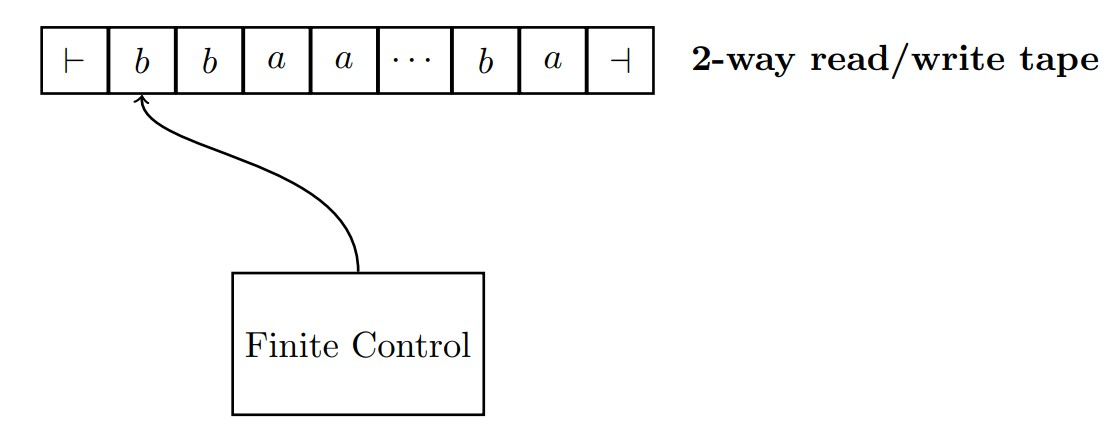
\includegraphics[scale=.5]{img5/m1}
	\caption{Linear Bounded Automata (LBA)}
\end{figure}
\end{frame}
\begin{frame}{Linear Bounded Automata (LBA)}
\textbf{Read/ write tape:}
\begin{itemize}
	\item Read/ write head can move to right/left, one cell at a time.
	\item The tape is initally assumed to be store the input delimited by $\dashv$ and the blank symbol $B$, which is followed by blank symbol ($\dashv$ )in all the cells until the cell containing $\vdash$
	\item If the input size is n, the number of cells in the tape which the machine can use is bounded by a linear function of n.
	\item The machine can scan the input in right/left directions any number of rounds
\end{itemize}
\textbf{Finite Control:}
\begin{itemize}
	\item Control unit with a finite set of states which can remember finite amount of information about the processed input.
\end{itemize}
\end{frame}
\begin{frame}{Linear Bounded Automata (LBA)}
	\textbf{Formal definition}
	\begin{itemize}
		\item Formally Linear Bounded Automata is a non-deterministic Turing	Machine, $M=(Q,\Sigma, \Gamma, \delta,B,\vdash,\dashv,q_0, t,r)$

		\begin{itemize}
			\item Q is set of all states
			\item $\Sigma$ is set of all terminals
			\item $\Gamma$ is set of all tape alphabets $\Sigma$ $\subset$ $\Gamma$
			\item $\delta$ is set of transitions $(Q\times \Gamma)\rightarrow (Q\times \Gamma \times \{R,L\})$
			\item $B$ is blank symbol ($B \in \Gamma$)
			\item $\vdash$ is left marker and $\dashv$ is right marker ($\vdash \ and\ \dashv\  \in \Gamma$)
			\item $q_0$ is the initial state ($q_0 \in Q$)
			\item $t$ is accept state ($t \in Q$)
			\item $r$ is reject state ($r \in Q$)
		\end{itemize}
	\end{itemize}
\end{frame}
\begin{frame}{Linear Bounded Automata (LBA)}
	\textbf{Example:}Consider an LBA defined as,
	\begin{eqnarray*}
		Q &=& \{q0, q1, q2, q3, q4\}\\
		\Sigma &=& \{a, b, c\}\\
		\Gamma &=& \{a, b, c, B\}
\\
		q0 &=& q0\\
				\delta(q0, \vdash) = (q1, \vdash, R)\ & \delta(q1, \vdash) = (q1, \vdash,R )\ & \delta(q1, B) = (q1, B, R) \\
		\delta(q1, a) = (q2, B, R )\ &  \delta(q2, a) = (q2, a, R)\ & \delta(q2, B) = (q2, B, R) \\
		\delta(q2, b) = (q3, B, R)\ & \delta(q3, b) = (q3, b, R)\ & \delta(q3, B) = (q3, B, R) \\
		\delta(q3, c) = (q4, B, L)\ & \delta(q4, c) = (q4, c, L)\ & \delta(q4, b) = (q4, b, L) \\
		\delta(q4, a) = (q4, a, L)\ & \delta(q4, B) = (q4, B, L)\ & \delta(q4, \dashv) = (q1, \vdash, R) 
	\end{eqnarray*}
	In the above, the transition $\delta(q3, b) = (q3, b, R)$ means,LBA on state q3, head points to symbol b, remains in state q3, replaces b with b and head turns towards right by one
	cell
\end{frame}
\begin{frame}{Linear Bounded Automata (LBA)}
	\textbf{Example:}1A.Design Linear Bounded Automata for the language $L = \{ a^n b^ n c^ n | n\geq1 \}$.
	\begin{eqnarray*}
		Q &=& \{q0, q1, q2, q3, t,r\}\\
		\Sigma &=& \{a, b, c\}\\
		\Gamma &=& \{a, b, c, X,Y,Z\}
		\\
		q0 &=& q0\\
		t = t (accept\  state) &,&
		r = r (reject\  state)\\
		\delta(q_0, \vdash) = (q_0, \vdash, R)\ & \delta(q_0, a) = (q_1, X,R )\ & \delta(q_1, a) = (q_1, a, R) \\
		\delta(q_1, b) = (q_2, Y, R )\ &  \delta(q_2, b) = (q_2, b, R)\ & \delta(q_2,c) = (q_3, Z, L) \\
		\delta(q_3, b) = (q_3, b, L)\ & \delta(q_3, Y) = (q|_3, Y, L)\ & \delta(q_3, a) = (q_3, a, L) \\
		\delta(q_3, X) = (q_0, X, R)\ & \delta(q_2, Z) = (q_2, Z, R)\ & \delta(q_3, Z) = (q_3, Z, L) \\
		\delta(q_1, Y) = (q_1, Y, R)\ & \delta(q_0, Y) = (q_0, Y, R)\ & \delta(q_0, Z) = (q_0, Z, R)  \\
		\delta(q_0, B) = (t, B, L)\ & \delta(q_0, b) = (r, b, R)\ & \delta(q_0, c) = (r, c, R)  \\
		\delta(q_1, c) = (r, c, R)\ & \delta(q_2, B) = (r, B, L)
	\end{eqnarray*}
\end{frame}
\section{Turing Machine (TM)}
\begin{frame}{Turing Machine (TM)}
	\begin{figure}
		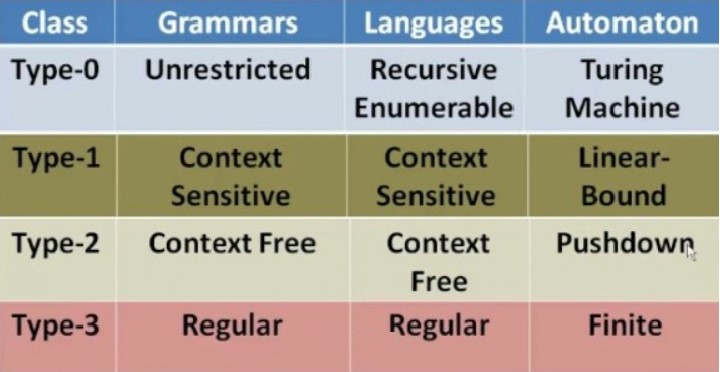
\includegraphics[scale=.5]{img5/m2}
		\caption{ Chomsky Hierarchy}
	\end{figure}
From the diagram, unrestricted grammars produce unrestricted languages (Type-0 languages). These Type-0 languages are recognised using Turing machines
\end{frame}
\begin{frame}{Turing Machine (TM)}
\textbf{Example of unrestricted grammars:}
\begin{eqnarray*}
	S &\rightarrow & ACaB \\
	CaBc &\rightarrow & aaC \\
	CB &\rightarrow & DB \\
	aD &\rightarrow & Da \\
	aEC &\rightarrow & Ea \\ 
	AE &\rightarrow & \epsilon \\
\end{eqnarray*}
Here LHS and RHS can contain any set of terminals and non terminals.
\end{frame}
\begin{frame}{Turing Machine (TM)}
	\begin{figure}
		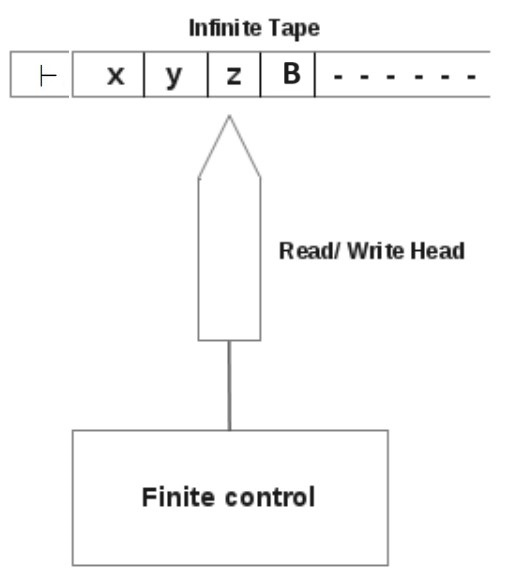
\includegraphics[scale=.45]{img5/m3}
		\caption{Turing Machine (TM)}
	\end{figure}
The basic model has a finite control, an input tape that is divided into cells, and a tape head that
scans one cell of the tape at a time. 
\end{frame}
\begin{frame}{Turing Machine (TM)}

\begin{itemize}
	\item Tape
\begin{itemize}
	\item The tape has a leftmost cell but is infinite to the right.
	\item  Each cell of the tape may hold exactly one 
	of a finite number of tape symbols.
	\item Initially, the n leftmost cells, for some finite $n\geq  0$, hold the input, which is a string of symbols 
	chosen from a subset of the tape symbols called the input symbols.
	\item The remaining infinity of cells each hold the blank, which is a special tape symbol that is not an 
	input symbol.
\end{itemize}
	\item Finite control
\begin{itemize}
	\item 	At a particular instant, finite control is in a state. States are divided into,
	\begin{itemize}
		\item Start state $(q0)$,
		\item Halt state $(h)$,
		\item Intermediate states $(q1, q2, .....)$.
	\end{itemize}
\end{itemize}
	\item Tape head
\begin{itemize}
	\item 	Tape head points to one of the tape cells. It communicates between finite control and tape. It can move left ,
	right or remain stationary.

\end{itemize}
\end{itemize}
\end{frame}
\begin{frame}{Turing Machine (TM)}
	\textbf{Moves of Turing Machine}\\
	In one move the Turing machine, depending upon the symbol scanned by the tape head and the state of 
	the finite control,
	\begin{enumerate}
		\item changes state
		\item prints a symbol on the tape cell scanned, replacing what was written there, and
		\item moves its head left or right one cell.
	\end{enumerate}
The difference between a Turing machine and a two-way finite automaton lies in the former's 
ability to change symbols on its tape.
\end{frame}	
\begin{frame}{Turing Machine (TM)}
	\textbf{Formal definition-Turing Machine (TM)}\\
	Turing Machine M is denoted by the 9-tuple: $M=(Q,\Sigma, \Gamma, \delta,B,\vdash,q_0, t,r)$
	
	\begin{itemize}
		\item Q is set of all states
		\item $\Sigma$ is a finite set (the input alphabet)
		\item $\Gamma$ is set of all tape alphabets $\Sigma$ $\subset$ $\Gamma$
		\item $\delta$ is set of transitions $(Q\times \Gamma)\rightarrow (Q\times \Gamma \times \{R,L\})$
		\item $B$ is blank symbol ($B \in \Gamma$)
		\item $\vdash$ is left marker  ($\vdash   \in \Gamma$)
		\item $q_0$ is the initial state ($q_0 \in Q$)
		\item $t$ is accept state ($t \in Q$)
		\item $r$ is reject state ($r \in Q$)
	\end{itemize}
Intuitively, $\delta (p, a) = (q, b, d)$ means, "When in state p scanning symbol a, 
write b on that tape cell, move the head in direction d(L/R), and enter state q.
The symbols Land R stand for left and right, respectively.
\end{frame}	
\begin{frame}{Turing Machine (TM)}
	\textbf{Instantaneous description (ID):}\\
	\begin{itemize}
		\item Instantaneous description of the Turing machine M is denoted by $\alpha_1q\alpha_2$
		\item Here q, the current state of M, is in $Q; \alpha_1\alpha_2$ is the string in $\Gamma^*$ that is the contents of the tape up to 
		the rightmost nonblank symbol or the symbol to the left of the head, whichever is rightmost. 
		(Observe that the blank B may occur in $\alpha_1\alpha_2$.)
		\item The tape head is assumed to be scanning the leftmost symbol of $\alpha_2$, or if $\alpha_2 = \epsilon$, the head is 
		scanning a blank.

	\end{itemize}
\end{frame}	
\begin{frame}{Turing Machine (TM)}
	\textbf{Define a move in TM}
	\begin{itemize}
		\item Let $X_1 X_2…X_{i-1} q X_i…X_n$ be an ID. 
		\item The left move is: if $\delta (q, X_i )= (p, Y,L)$ ,if $i>1$ then
		\begin{itemize}
			\item $X_1 X_2…X_{i-1} q X_i…X_n \vdash X_1X_2… X_{i-2} p X_{i-1} Y X_{i+1}…X_n.$ 
		\end{itemize}
		\item The right move is: if $\delta (q, X_i )= (p, Y,R)$ ,if $i>1$ then
		\begin{itemize}
			\item $X_1 X_2…X_{i-1} q X_i…X_n \vdash X_1X_2… X_{ i-1}Y p X_{i+1}…X_n.$ 
		\end{itemize}
		
	\end{itemize}
\end{frame}	
\begin{frame}{Turing Machine (TM)}
	\textbf{Language accepted by a turing machine}\\
	The language of a Turing machine M, denoted L(M), is 
	the set of all strings that M accepts:
	$$L(M) = \{ w \in \Sigma^* | M\  accepts\  w \}$$
	
	TM either accepts or rejects a string. That is, \textbf{TM acts as a language acceptor.}

	\begin{itemize}
		\item A TM is said to accept an input string w if : $(q_0,\vdash w B^W,0) \xRightarrow *(t,y,n),y\in \Gamma^w,n\in  N$
			\item A TM is said to reject an input string w if : $(q_0,\vdash w B^W,0) \xRightarrow *(r,y,n),y\in \Gamma^w,n\in  N$
	\end{itemize}
\end{frame}	
\subsection{Turing Machines as Language Accepters}
\begin{frame}{Turing Machines as Language Accepters}
\textbf{Turing Machines as Language Accepters}
\begin{itemize}
	\item Turing machines can be viewed as accepters in the following sense.
	\begin{itemize}
		\item String w is written on the tape, with blanks filling out the unused
		portions. 
		\item The machine is started in the initial state $q_0$ with the read-write head positioned on the leftmost symbol of w.
		\item If, after a sequence	of moves, the Turing machine enters a final state and halts, then w is
		considered to be accepted.
	\end{itemize} 
\textbf{Definition}
\begin{itemize}
	\item Let $M=(Q,\Sigma, \Gamma, \delta,B,\vdash,q_0, t,r)$ be a Turing machine. Then the language accepted by M is 	$$L (M) = \{w \in \Sigma^+: q_0w\vdash^*x_1q_f x_2\ for\  some\  q_f \in t, x_1,x_2 \in \Gamma^*\}.$$
\end{itemize}
	
\end{itemize}
\end{frame}
\begin{frame}{Turing Machine (TM)}
\textbf{Q:}Design a TM to accept the language $L = \{0^n1^n	| n\geq 1\}.$
\begin{itemize}
	\item Initially, the tape of M contains $0^n1^n$
	followed by infinity of blanks. 
	\item Repeatedly, M replaces the leftmost 0 by X, moves right to the leftmost 1, replacing it by Y, moves left 
	to find the rightmost X, then moves one cell right to the leftmost 0 and repeats the cycle.
	\item If, however, when searching for a 1, M finds a blank instead, , then M halts without accepting. 
	\item If, after changing a 1 to a Y, M finds no more 0's, then M checks that no more 1's remain, accepting if 
	there are none
\end{itemize}

\end{frame}	
\begin{frame}{Turing Machine (TM)}
\begin{figure}
	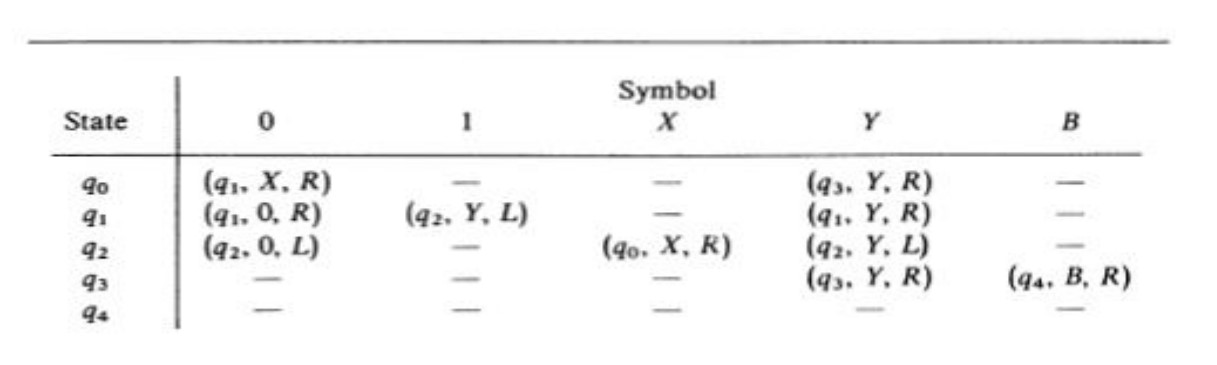
\includegraphics[scale=.45]{img5/m4}
	\caption{Transition table}
\end{figure}
\end{frame}	
\begin{frame}{Turing Machine (TM)}
	\begin{figure}
		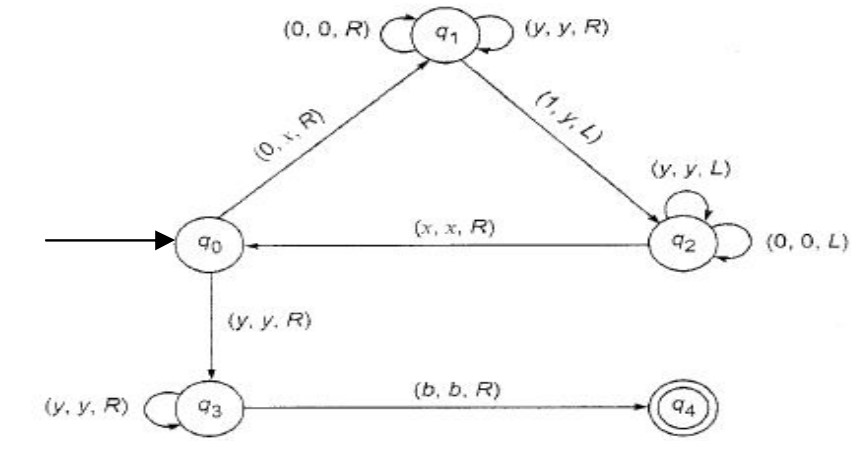
\includegraphics[scale=.45]{img5/m5}
		\caption{Transition diagram}
	\end{figure}
\end{frame}	
\begin{frame}{Turing Machine (TM)}
	String Verfication by Turing Machine
	\begin{figure}
		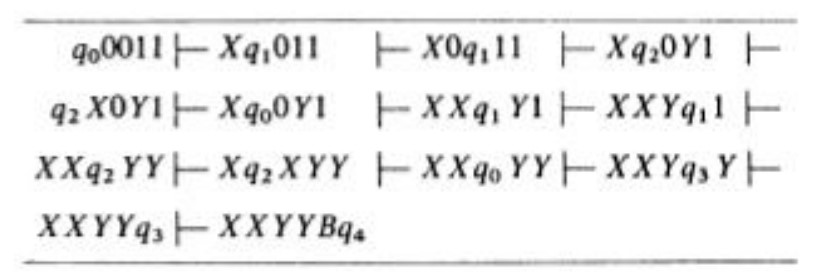
\includegraphics[scale=.45]{img5/m6}
		\caption{A computation of M}
	\end{figure}
\end{frame}	
\subsection{Turing Machine as Transducers}
\begin{frame}{Turing Machine (TM)}
\textbf{TM as transducers}\\
A TM can function as a transducer. That is, a string is given as input to TM, it produces some output.
\begin{itemize}
	\item Input to the computation is a set of symbols on the tape.
	\item At the end of computation, whatever remains on the tape is the output.
\end{itemize}
A TM can be viewed as a transducer for the implementation of function f defined as,$y=f(x)$ for strings $x, y\in \Sigma^*$
\begin{itemize}
	\item A function, f is said to be computable or Turing computable, if there exists a TM M such that $q_0 x \vdash^* q_f\  f(x)$
	\item where x is in the domain of f.
\end{itemize}
\end{frame}	

\begin{frame}{Turing Machine (TM)}
	\textbf{TM is an abstract model of our modern computer system}
	\begin{itemize}
		\item 	We can see that all common mathematical functions are turing computable.
		\item This means, basic operations such as addition, subtraction, multiplication, division can be performed on it.
		\item This means that a TM is an abstract model of our modern computer system.
	\end{itemize}

\end{frame}		
\begin{frame}{Turing Machine (TM)}
	\textbf{Unary Representation}
	\begin{itemize}
		\item In computing functions using a Turing machine (TM) where inputs are represented using unary notation, a non-negative integer n is indeed represented as a sequence of 1s or 0s.
		\item For example:
		\begin{itemize}
			\item If n = 2, it is represented as "11" or "00"
		\item	If n = 4, it is represented as "1111" or "0000"
		\end{itemize}
	\end{itemize}
\end{frame}	
\begin{frame}{Turing Machine (TM)}
	\textbf{Q:}Design a Turing machine that computes the following function, $$f(m, n) = m + n.$$
		A positive integer on a Turing tape can be represented by an equal number of 0s.For example,
		\begin{itemize}
			\item integer 5 is represented as 00000, and
		\item integer 8 is represented as 00000000.
		\end{itemize}
	In the tape two integers are separated using the symbol, $\$ $.\\

	
\end{frame}	
\begin{frame}{Turing Machine (TM)}
	Let us assume that m=3 and n=5.Then the input tape of the Turing machine will be,
\begin{figure}
	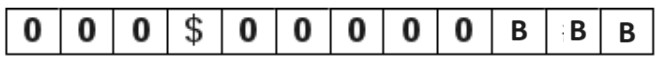
\includegraphics[scale=.45]{img5/m7}
%	\caption{A computation of M}
\end{figure}
After addition, tape will contain the results of addition as shown below
\begin{figure}
	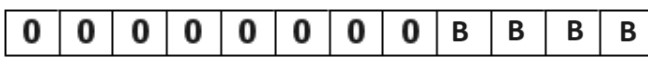
\includegraphics[scale=.45]{img5/m8}
	%	\caption{A computation of M}
\end{figure}
TM for addition works as follows:
\begin{itemize}
	\item Head reads the 0s of the first number, m and reaches the separator symbol, $\$ $. Symbol, $\$ $ is replaced with 0 and head
	moves towards right
	\item It continues to move towards right till the second number, n is passed over and B is reached.
	\begin{itemize}
		\item At B, it turns left and replaces rightmost 0 with B.
		\item Now the tape contains the sum of m and n, and TM halts.
	\end{itemize}
\end{itemize}
\end{frame}	
\begin{frame}{Turing Machine (TM)} 
Conversion of the separator symbol, $\$ $ to 0, helps TM to make the single number on the tape. The conversion of symbol,
0 to B removes the additional 0 that was generated from the conversion of $\$$ to 0.\\
Transition table for the TM is shown below:
\begin{figure}
	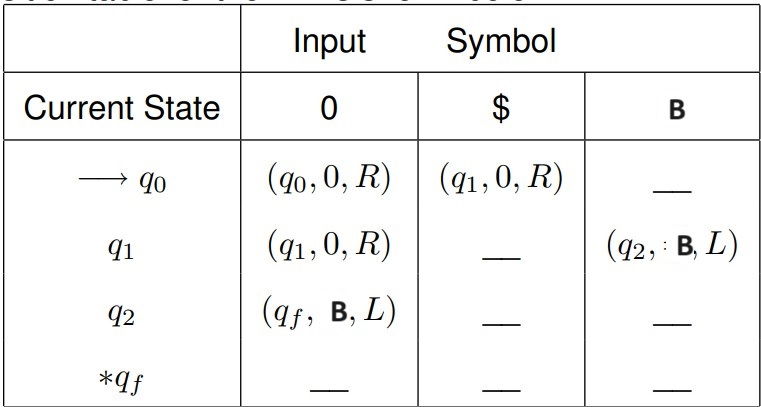
\includegraphics[scale=.45]{img5/m9}
		\caption{Transition table}
\end{figure}
\end{frame}	
\begin{frame}{Turing Machine (TM)} 
The Transition table  is describes as follows:
\begin{enumerate}
	\item  Initially, TM is in state $q_0$. Head reads the first symbol, 0 and moves towards right without changing the state.
	\item Head continues to move towards right till the separator symbol,$\$ $ is reached. It replaces $ \$ $ with 0, changes state to
	q1, and continues to move towards right.
	\item Head continues to move towards right and passes over the second number to reach B.
	\item On reaching the B, head changes state to $q_2$ and turns left.
	\item In state $q_2$, it replaces symbol 0 with B, and changes state to $q_f$ .
	\item In the final state, TM halts to indicate the completion of the process.

\end{enumerate}
\end{frame}	
\begin{frame}{Turing Machine (TM)} 
	Addition of 3 and 5 is shown below
\begin{figure}
	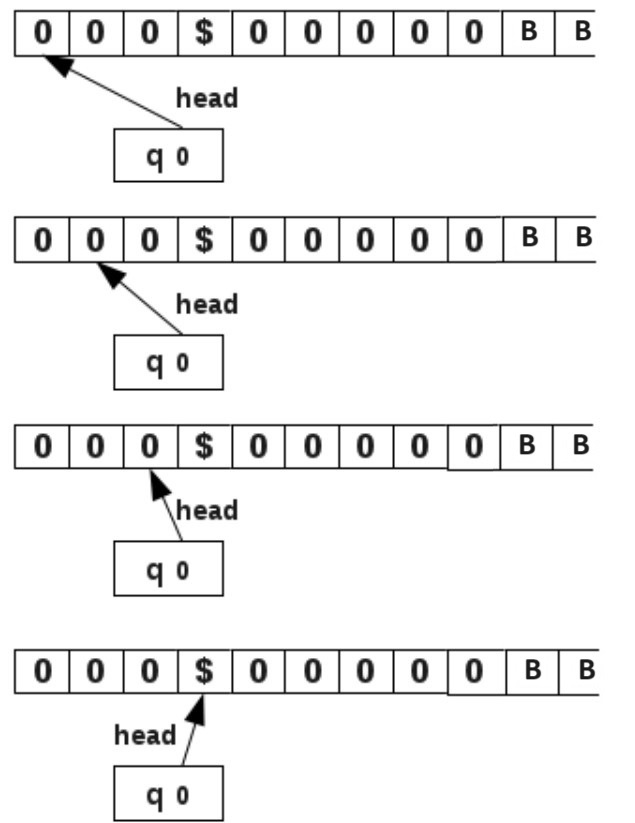
\includegraphics[scale=.4]{img5/m10}
%	\caption{Transition table}
\end{figure}
\end{frame}	
\begin{frame}{Turing Machine (TM)} 
	\begin{figure}
		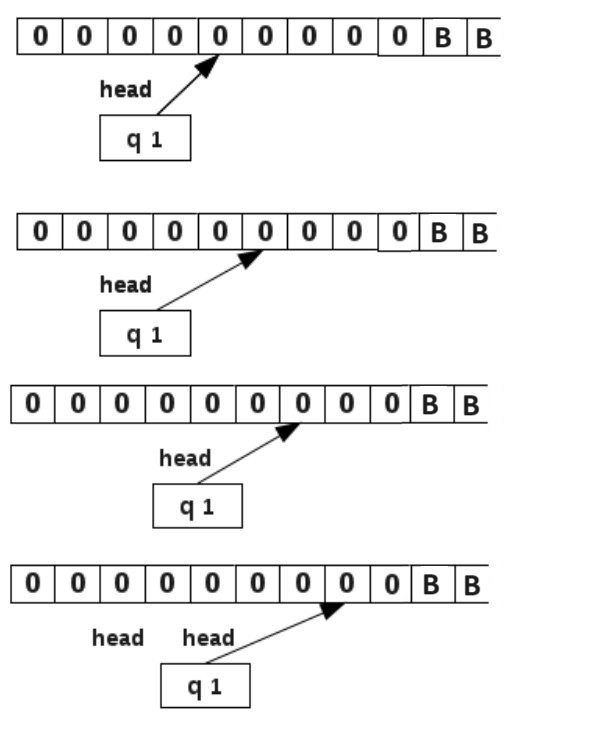
\includegraphics[scale=.45]{img5/m11}
		%	\caption{Transition table}
	\end{figure}
\end{frame}	
\begin{frame}{Turing Machine (TM)} 
	\begin{figure}
		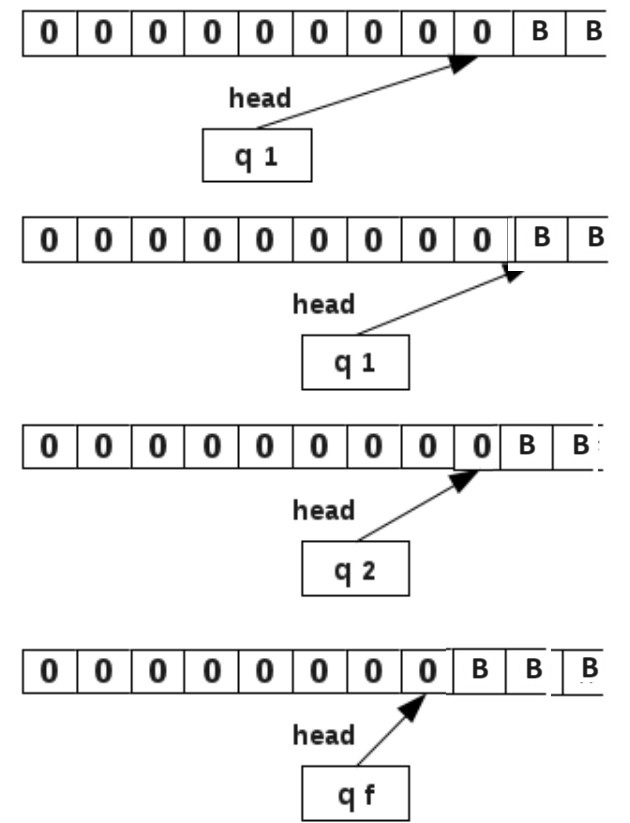
\includegraphics[scale=.4]{img5/m12}
		%	\caption{Transition table}
	\end{figure}
\end{frame}	
\section{Robustness of the standard TM model}
\begin{frame}{Robustness of the standard TM model}
\textbf{Robustness of the standard TM model}
\begin{itemize}
	\item A computational model is robust if the class of languages it
	accepts does not change under variants.
	\item The robustness of Turing Machines is by far greater than
	the robustness of DFAs and PDAs.

	\item We introduce several variants on Turing machines and show
	that all these variants have equal computational power.

\end{itemize}
\end{frame}
\begin{frame}{Robustness of the standard TM model}
	\textbf{Types of Turing Machines}
	\begin{itemize}
		\item Two-way infinite tape
		\item Multitape Turing machines
		\item Multi-track Turing Machine
		\item Nondeterministic Turing machines
		\item Multidimensional Turing machines
		\item Off-line Turing machines
		\item Universal Turing Machines
	\end{itemize}
\end{frame}
\begin{frame}{Two-way infinite tape}
	\textbf{Two-way infinite tape}
	\begin{itemize}
		\item The TM we discussed so far had a tape that was finite on the left end and infinite on the right end.
		\item Two way infinite TM is an extension to this such that tape is infinite at both ends. This is shown below:
\begin{figure}
	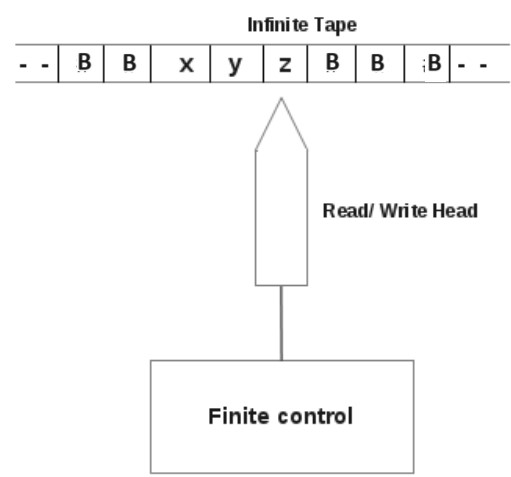
\includegraphics[scale=.34]{img5/m13}
		\caption{Two-way infinite tape}
		\small \begin{itemize}
			\item Thus on both sides of the tape, there is an infinite sequence of blank symbols(B).
		\item This model does not provide any additional computational capability.
		\end{itemize}
\end{figure}
\end{itemize}
\end{frame}

\section{Multitape Turing Machines}
\begin{frame}{ Multitape Turing Machines}
	\textbf{ Multitape Turing Machines}
	\begin{itemize}
		\item A multitape TM consists of multiple tapes. Each tape has a separate head
	\end{itemize}
\begin{figure}
	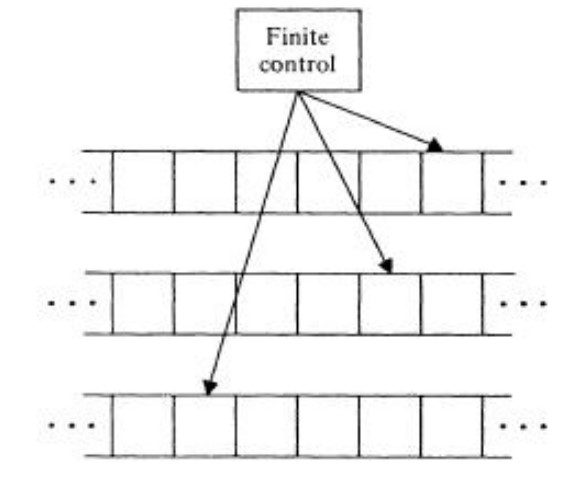
\includegraphics[scale=.4]{img5/m14}
	\caption{Multitape Turing Machines}
\end{figure}
\end{frame}
\begin{frame}{ Multitape Turing Machines}
	\textbf{ Multitape Turing Machines}
	\begin{itemize}
		\item There are n tapes, each divided into cells. The first tape holds the input string. Initially, all the other tapes hold the blank
		symbol, B
		\item A head has three possible options:
		\begin{itemize}
			\item to move towards left (L),
			\item to move towards right (R), or
			\item to remain stationary (N).
		\end{itemize}
	\item All the heads are connected to a finite control. Finite control is in a state at an instant.
	\begin{enumerate}
		\item Initially, finite control is in state $q_0$.
		\item Head in the lowermost tape points to the cell containing leftmost symbol of the input string.
		\item All the cells in the upper tapes contain B symbol
	\end{enumerate}
	\end{itemize}
\end{frame}
\begin{frame}{ Multitape Turing Machines}
	\begin{itemize}
		\item When a transition occurs,
		\begin{enumerate}
			\item Finite control may change its state.
			\item Head reads the symbol from the current cell and writes a symbol on it.
			\item Each head can move towards left (L), right (R) or stay stationary (N)
		\end{enumerate}
	\end{itemize}
An example transition function for a 4 tape TM is given below:
\begin{itemize}
	\item $\delta(q_1, [a_1, a_2, a_3, a_4]) = (q_2, [b_1, b_2, b_3, b_4], [L, R, R, N])$
	\item Here the finite control is in state $q_1$, It reads the symbol $a_1$ from the uppermost tape, $a_2$ from the next uppermost tape and so on.
  \item After reading, finite control changes its state to $q_2$, and replaces the symbol $a_1$ by $b_1$, $a_2$ by $b_2$, $a_3$ by $b_3$ , $a_4$ by $b_4$.
\item After this head in the upper most tape turns left.
 Head in the 2nd tape turns right. Head in the 3rd tape turns right. Headin the 4th tape remains stationary.

\end{itemize}
\end{frame}
\begin{frame}{ Multitape Turing Machines}
\textbf{Example:}Consider the language $L = \{a^nb^n \big |n \geq 1\}.$

\begin{itemize}
	\item In a normal TM, head has to move back and forth to match each pair of symbols a and b. On a multitape TM, no such	movements are needed.
	\item This is done by making a copy of the input string in another tape.
	\item Let the input string be aaaabbbb.
	\item Let the input srtring be in tape 1. Make a copy of this string in tape 2
\end{itemize}
\begin{figure}
	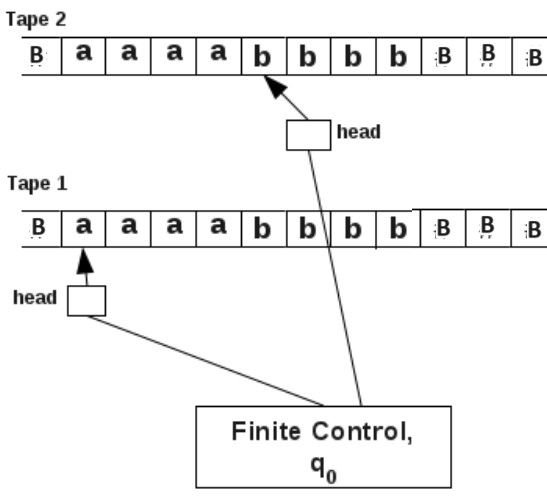
\includegraphics[scale=.4]{img5/m15}
	\caption{Multitape Turing Machines}
\end{figure}
\end{frame}
\begin{frame}{ Multitape Turing Machines}
\begin{itemize}
	\item The head of tape 1 is positioned on the first a of the input string. Head of tape 2 is positioned on the first b of the input
	string.
	\item Now the heads advance on both tapes simultaneously towards right and the string is accepted if there are equal number
	of a’s and b’s in the string.
	\item This will happen if the head on tape 1 encounters the first b and the head on tape 2 encounters the first B(blank symbol) simultaneously.
\end{itemize}
\textbf{$^*$}Every multitape Turing Machines has an equivalent single tape Turing
machine.

\end{frame}
\begin{frame}{Multi-track Turing Machine}
	\textbf{Multi-track Turing Machine}
	\begin{itemize}
		\item Multi-track Turing machines, a specific type of Multi-tape Turing machine, contain
		multiple tracks but just one tape head reads and writes on all tracks. \item Here, a single
		tape head reads n symbols from n tracks at one step. 
		\item It accepts recursively
		enumerable languages like a normal single-track single-tape Turing Machine accepts.
	\end{itemize}
\begin{figure}
	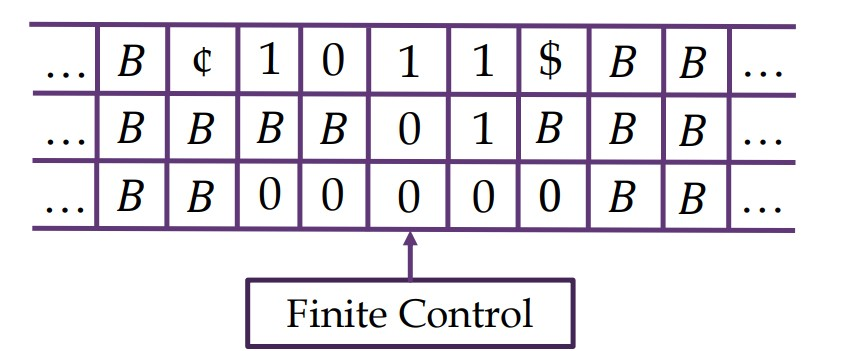
\includegraphics[scale=.4]{img5/m16}
	\caption{Multi-track Turing Machines}
\end{figure}
\end{frame}

\begin{frame}{ Multitape Turing Machines}
\textbf{Theorem:}\\ Every language accepted by a k-tape TM M1 is also accepted by a single tape TM M2\\
\textbf{Proof by construction}
	\begin{itemize}
		\item Let L be accepted by M1 ,a TM with k-tapes. We can construct M2, a one-tape TM with 2k tracks, two tracks for each of M1’s tapes.
		\item One track records the contents of the corresponding tape of M1
		\item and the other is blank, except for a marker in the cell that holds the symbol scanned by the corresponding head of M1.
		\item  The finite control of M2 stores the state of M1 ,along with a count of the number of head markers to the right of M2’s tape head.H
	\end{itemize}
\end{frame}
\begin{frame}{ Multitape Turing Machines}
	\begin{figure}
		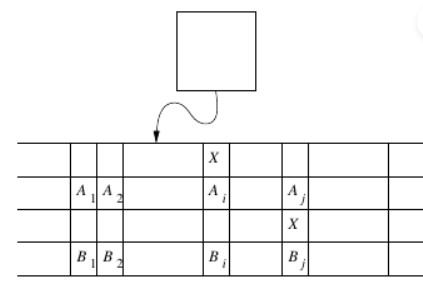
\includegraphics[scale=.8]{img5/m18}
		\caption{Simulation of multi tapes by one}
	\end{figure}
\end{frame}
\begin{frame}{ Multitape Turing Machines}
	\textbf{To simulate one move of the k-tape TM:}
	\begin{itemize}
		\item Each move of M1 is simulated by a sweep from left to right and then from right to left by the tape head of M2.
		\item Initially, M2’s head is at the leftmost cell containing a head marker.
		\item To simulate a move of M1, M2 sweeps right, visiting each of the celis with head markers andrecording the symbol scanned by each head of M1.
		\item When M2 crosses a head marker, it mustupdate the count of head markers to its right.
		\item When no more head markers are to the right, M2 has seen the symbols scanned by each of M1’s heads, so M2 has enough information todetermine the move of M1.
		\item  Now M2 makes a pass left, until it reaches the leftmost headmarker.
	\end{itemize}
\end{frame}
\begin{frame}{ Multitape Turing Machines}
	\begin{itemize}
		\item The count of markers to the right enables M2 to tell when it has gone for enough.
		\item  As M2 passes each head marker on the leftward pass, it updates the tape symbol of M1 “scanned”by that head marker, and it moves the head marker one symbol left or right to simulate themove of M1.
		\item  Finally, M2 changes the state of M1 recorded in M2’s control to complete thesimulation of one move of M1.
		\item   If the new state of M1 is accepting, then M2 accepts.
	\end{itemize}
\end{frame}
\section{Nondeterministic Turing machines}
\begin{frame}{Nondeterministic Turing machines}
\textbf{Nondeterministic Turing machines}
\begin{itemize}
	\item A nondeterministic Turing machine is a device with a finite control and a single, one-way infinite 
	tape.
	\item For a given state and tape symbol scanned by the tape head, the machine has a finite number of 
	choices for the next move.
	\item Each choice consists of a new state, a tape symbol to print, and a direction 
	of head motion.
	\item Note that the nondeterministic TM is not permitted to make a move in which the next 
	state is selected from one choice, and the symbol printed and/or direction of head motion are selected 
	from other choices.
	\item The nondeterministic TM accepts its input if any sequence of choices of moves leads to an accepting state.
	
\end{itemize}
\end{frame}

\begin{frame}{Nondeterministic Turing machines}
	\textbf{Formal definition- Nondeterministic Turing Machine}\\
Nondeterministic Turing Machine M is denoted by the 9-tuple: $M=(Q,\Sigma, \Gamma, \delta,B,\vdash,q_0, t,r)$

\begin{itemize}
	\item Q is set of all states
	\item $\Sigma$ is a finite set (the input alphabet)
	\item $\Gamma$ is set of all tape alphabets $\Sigma$ $\subset$ $\Gamma$
	\item $\delta$ is set of transitions $(Q\times \Gamma)\rightarrow 2^{(Q\times \Gamma \times \{R,L\})}$
	\item $B$ is blank symbol ($B \in \Gamma$)
	\item $\vdash$ is left end marker  ($\vdash   \in \Gamma$)
	\item $q_0$ is the initial state ($q_0 \in Q$)
	\item $t$ is accept state ($t \in Q$)
	\item $r$ is reject state ($r \in Q$)
	\item $t,r \in Q$ are sink states
\end{itemize}
\end{frame}
\begin{frame}{Nondeterministic Turing machines}
	\begin{figure}
		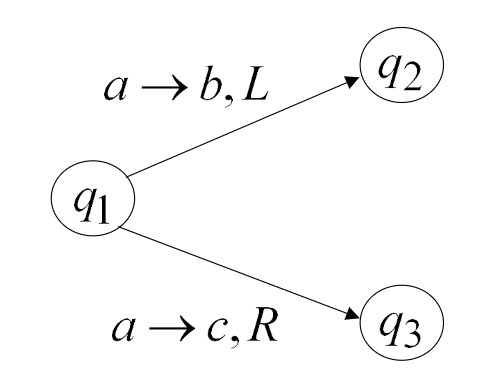
\includegraphics[scale=.4]{img5/m17}
		\caption{Nondeterministic Turing machine}
	\end{figure}
\end{frame}
\begin{frame}{Nondeterministic Turing machines}
Every nondeterministic Turing Machine has an equivalent deterministic Turing machine\\
	\textbf{Theorem}
	\begin{itemize}
		\item If L is accepted by a single-tape NDTM $M_1$, then L is accepted by some DTM $M_2$.
	\begin{itemize}
	\item Let d be the maximum number of nondeterministic 
		choices $M_1$ can make at any given move.
			\item 	 $M_2$ will systematically try all nondeterministic 
		possibilities.
			\item 	 $M_2$ will have three tapes.
	\end{itemize}
\item $M_2$ uses 3 tapes:
\begin{itemize}
	\item Tape 1 holds the input,It’s reused many
	times.
	\item Tape 2 contains a sequence of digits from 1 to d, 
	generated systematically. Each sequence dictates a 
	sequence of choices. eg: 
	 \begin{itemize}
	 	\item[.]  [1 ],[ 2 ], [3 ], ... , [d] ,
	 	\item[.]  [1,1] , [1, 2] , [2, 1] , ... , [d, d] ,
	 	\item[.]  [1,1,1] , [1,1,2 ], [1, 2, 1] , ... , [d, d, d] ,
	 \end{itemize}
 \item Tape 3 contains a scratch copy of the input.
\end{itemize}
	\end{itemize}
\end{frame}
\begin{frame}{Nondeterministic Turing machines}
	\begin{figure}
		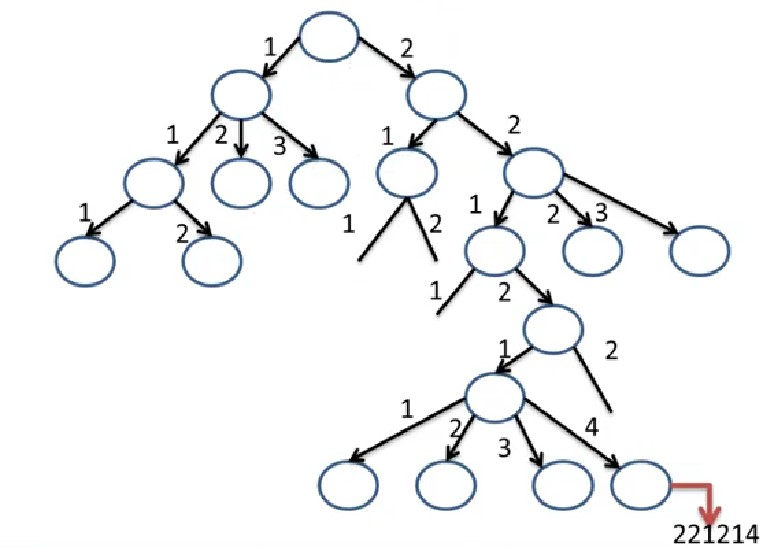
\includegraphics[scale=.5]{img5/m20}
		\caption{The computational tree of a non-deterministic Turing machine}
	\end{figure}
\end{frame}
\begin{frame}{Nondeterministic Turing machines}
		\begin{figure}
		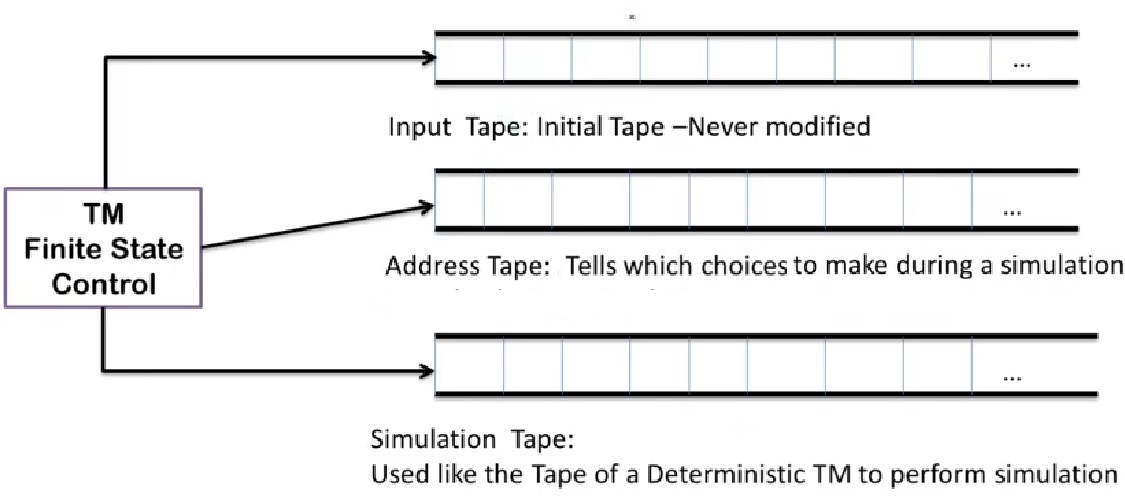
\includegraphics[scale=.5]{img5/m19}
		\caption{Deterministic TM simulating Nondeterministic Turing machine}
	\end{figure}
\end{frame}
\begin{frame}{Nondeterministic Turing machines}
	How $M_2$ works :
	\begin{enumerate}
		\item Generate the next sequence on tape 2
		\item Copy tape 1 (input) to tape 3 (scratch copy)
		\item Simulate $M_1$ on tape 3, making choices according 
		to the sequence on tape 2.
		\item If $M_1$ accepts, then accept;
		\item Otherwise, go to step 1.
	\end{enumerate}
\end{frame}
\section{Universal Turing Machines}
\begin{frame}{Universal Turing Machines}
	\textbf{Universal Turing Machines}
	\begin{itemize}
		\item A Turing machine (TM) U is called a universal Turing machine (UTM) if it is able to simulate
		all other TMs: 
		\item for all TMs M and inputs w, $U(<M, w>) = M(w).$
		\item A Universal turing Machine (UTM) takes two arguments 
		\begin{enumerate}
			\item The description of a normal TM
			\item The description of input string w and checks whether w is recognised
				\end{enumerate} 
		\item  The description of TM and input string w is the encoded string over a finite alphabet set.
	\end{itemize}

\end{frame}
\begin{frame}{Universal Turing Machines}
	\textbf{Unary Encoding of the elements in a turing machine}
	\begin{figure}
	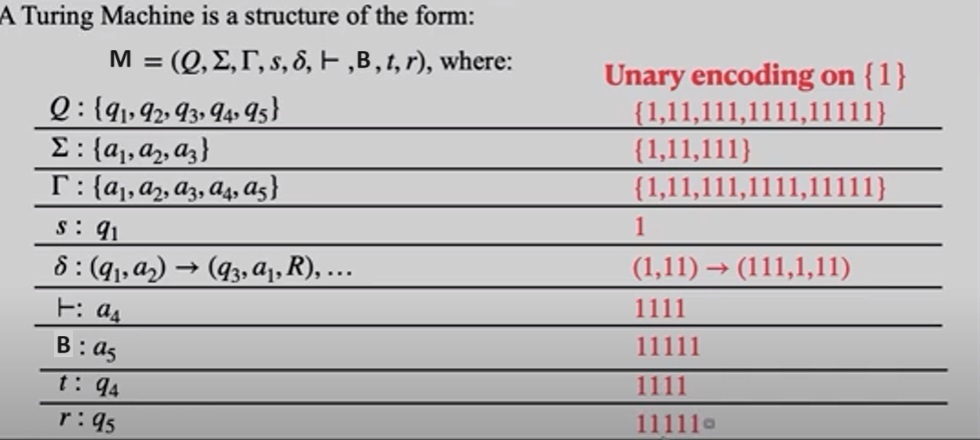
\includegraphics[scale=.6]{img5/m21}
	%\caption{Deterministic TM simulating Nondeterministic Turing machine}
\end{figure}
\end{frame}
\begin{frame}{Universal Turing Machines}
	\textbf{Total coding(Binary Encoding) of the TM is}
	\begin{figure}
		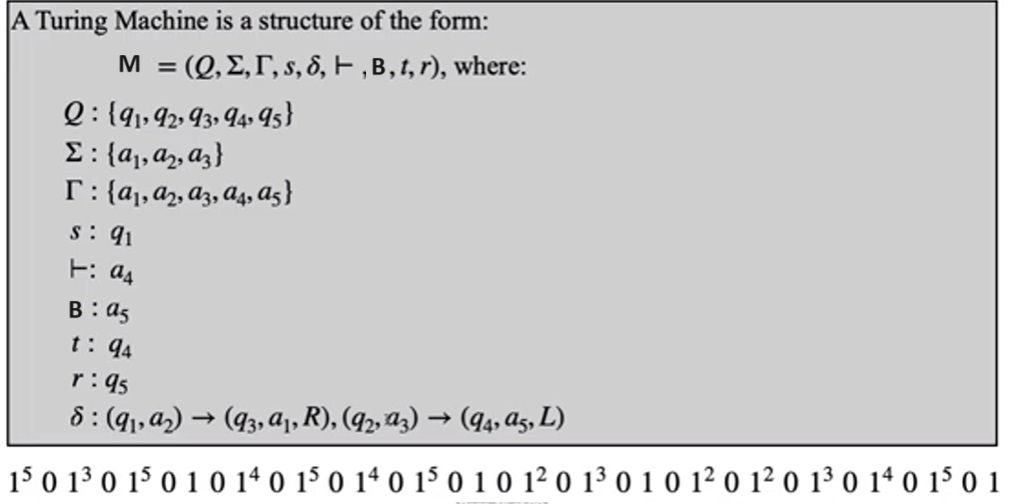
\includegraphics[scale=.55]{img5/m22}
		%\caption{Deterministic TM simulating Nondeterministic Turing machine}
	\end{figure}
\end{frame}
\begin{frame}{Universal Turing Machines}
	\textbf{Encoding of an input string}
	\begin{itemize}
		\item Consider $\Sigma = \{a,b\}$
		\item Using unary encoding on the alphabet set $\{1\}$
		\begin{itemize}
			\item a can be represented as 1 and
			\item b can be represented  as 11.
		\end{itemize}
	\item and each successive character representations are separated with a 0
		\item 	Let $w = abab$  be the string to be checked on the Turing machine, M. The input to UTM will be
		\begin{itemize}
			\item $\hat{w} = 101101011$
		\end{itemize}
	\item UTM uses the binary code of the turing machine, M on string abab and will check if abab is recognised by M. If true
	UTM, will halt to say yes and if false UTM will stop to say no.

	\end{itemize}

\end{frame}
\begin{frame}{Universal Turing Machines}
%	\textbf{Total coding(Binary Encoding) of the TM is}
	\begin{figure}
		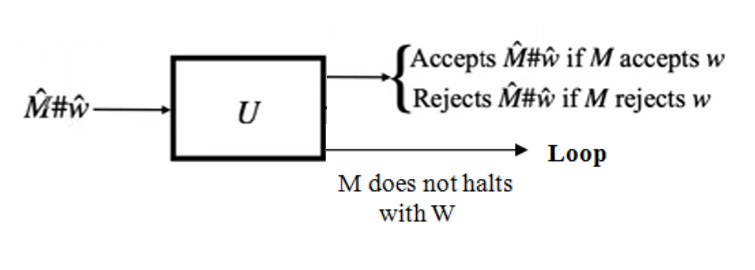
\includegraphics[scale=.55]{img5/m23}
		\caption{Universal Turing Machines}
	\end{figure}
	\begin{figure}
	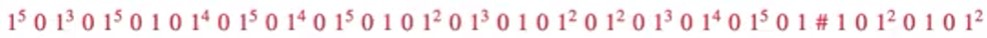
\includegraphics[scale=.55]{img5/m24}
	\caption{Input to Universal Turing Machines}
\end{figure}
\end{frame}
\begin{frame}{Universal Turing Machines}
\begin{itemize}
	\item U takes as input the binary encoding $\hat{M}$ of turing Machine M and the binary encoding $\hat{w}$ of an input w to M, seperated by a $\#$\  $(\Sigma_U = \{0,1,\#\})$
	\item Given the input string $\hat{M}\#\hat{w}$:
	\begin{itemize}
		\item Checks whether $\hat{M}$ is a valid encoding of a Turing Machine and $\hat{w}$ is a valid encoding of a string. Rejects if encoding is not valid
		\item Run M on w and:
		\begin{itemize}
			\item[a] Accepts if M accepts w.
			\item[b] Rejects if M rejects w.
			\item[c] Loops if M loop on w
		\end{itemize}
	\end{itemize}
\end{itemize}
\end{frame}
\begin{frame}{Universal Turing Machines}
		\begin{figure}
		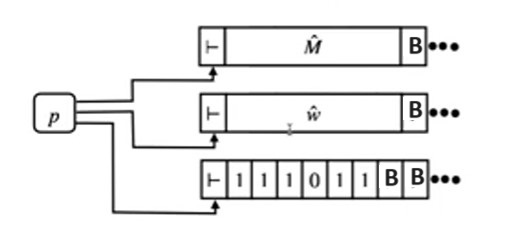
\includegraphics[scale=.75]{img5/m25}
		\caption{Structure of a UTM}
	\end{figure}
\begin{itemize}
	\item Tape 1 storing the encoding $\hat{M}$ of the TM M
	\item Tape 2 storing the encoding $\hat{w}$ of the i/p w
	\item Tape 3 storing the Current state of M and the current position of tape head in M
\end{itemize}
\end{frame}
\begin{frame}{Universal Turing Machines}
	\begin{itemize}
		\item U repeatedly performs the following, to simulate a single step of M on w:
		\begin{enumerate}
			\item Scan tape 3 and find M's current state and the current position of the tape head.
			\item Scan tape 2 and find the next input symbol of M
			\item Scan tape 1 and find the transition to apply in the current configuration of M.
			\item Apply the transition in the current configuration of M and accordingly , update tape2 and 3
			\item If M enters $t_M \big| r_M $ then enter $t_U \big| r_U $
		\end{enumerate}
	\end{itemize}
\end{frame}
\section{Halting Problem of TM}
\begin{frame}{Halting Problem of TM}
\textbf{Halting Problem of TM}
\begin{itemize}
	\item In computability theory, the halting problem is the problem of determining,
	from a description of an arbitrary computer program and an input, whether the
	program will finish running, or continue to run forever.
\item Alan Turing proved in 1936 that a general algorithm to solve the halting
	problem for all possible program-input pairs cannot exist.
\item Halting problem is undecidable.
\end{itemize}
\end{frame}
\begin{frame}{Halting Problem of TM}
	\textbf{Problem}
	\begin{itemize}
		\item Given the description of a Turing machine M and an input w, does M, when
		started in the initial configuration $q_0w$, perform a computation that eventually
		halts?
		\item \textbf{Input:}  A Turing machine and an input string w.
		\item \textbf{Problem:} Does the Turing machine finish computing of the string w in a finite	number of steps? The answer must be either yes or no
	\end{itemize}
\end{frame}
\begin{frame}{Halting Problem of TM}
	\textbf{Proof:}
	\begin{itemize}
		\item At first, we will assume that such a Turing machine exists to solve
		this problem and then we will show it is contradicting itself.
		\item We will call this Turing machine as a Halting machine that produces a
		‘yes’ or ‘no’ in a finite amount of time.
		\item If the halting machine finishes in a finite amount of time, the output comes
		as ‘yes’, otherwise as ‘no’.
		\item The following is the block diagram of a Halting machine.
	\end{itemize}
\begin{figure}
	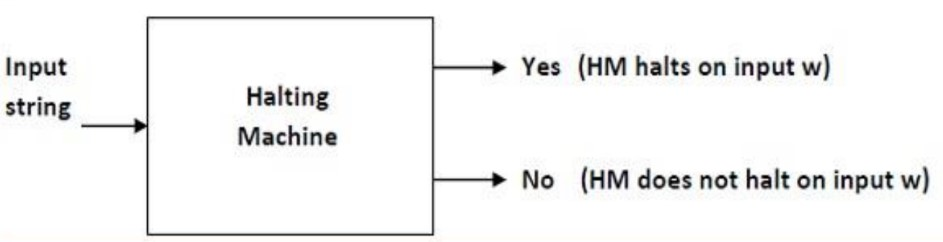
\includegraphics[scale=.5]{img5/m26}
	\caption{Halting machine}
\end{figure}
\end{frame}
\begin{frame}{Halting Problem of TM}
	\textbf{Proof cont..}
	\begin{itemize}
		\item Now we will design an inverted halting machine (HM)’ as
		\begin{itemize}
			\item If H returns YES, then loop forever.
			\item If H returns NO, then halt.
		\end{itemize}
	\item The following is the block diagram of an ‘Inverted halting machine’
	\end{itemize}
	\begin{figure}
		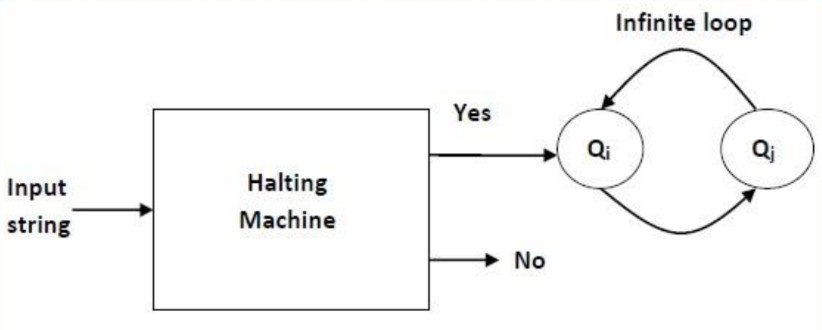
\includegraphics[scale=.5]{img5/m27}
		\caption{Inverted halting machine (HM)’}
	\end{figure}
\end{frame}
\begin{frame}{Halting Problem of TM}
	\textbf{Proof cont..}
	\begin{itemize}
		\item Further, a machine $HM_2$ which input itself is
		constructed as follows
		\begin{itemize}
			\item If $HM_2$ halts on input, loop forever.
			\item Else, halt.
		\end{itemize}
		\item Here, we have got a contradiction. Hence, the
		halting problem is undecidable.
	\end{itemize}
	\begin{figure}
		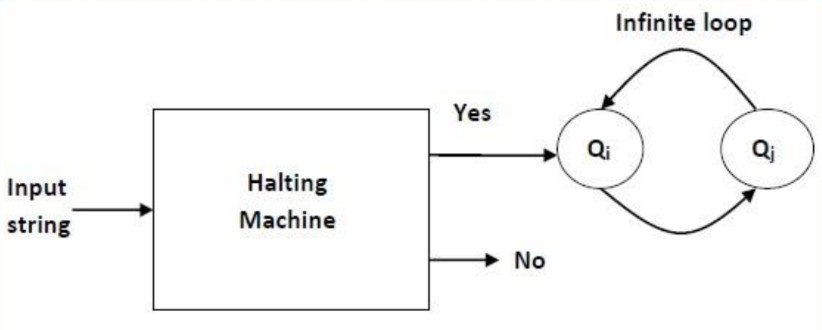
\includegraphics[scale=.5]{img5/m27}
		\caption{Inverted halting machine (HM)’}
	\end{figure}
\end{frame}
\section{Recursive and Recursive Enumerable Language}
\begin{frame}{Recursive and Recursive Enumerable Language}
\textbf{Recursive set}
\begin{itemize}
	\item A set is called recursively enumerable if there's a step-by-step method, like using a specific rule or algorithm, that can eventually list out all the numbers in that set.
	\item However, this method might take a while, and it can't quickly tell you whether a specific number is in the set or not. So, it's a way to gradually list the numbers but not a straightforward way to decide if a particular number belongs to the set.
	\item The union and intersection of two recursively enumerable sets are also recursively enumerable.
\end{itemize}
\end{frame}
\begin{frame}{Recursive and Recursive Enumerable Language}
	\textbf{Recursive set}
	\begin{itemize}
		\item A set S of integers is said to be recursive if there is a total recursive function $f(x)$ such that $f(x)=1$ for x in S and $f(x)=0$ for x not in S. 
		\item Any recursive set is also recursively enumerable.
		\item Finite sets, sets with finite complements, the odd numbers, and the prime numbers are all examples of recursive sets.
		\item The union and intersection of two recursive sets are themselves recursive, as is the complement of a recursive set.
	\end{itemize}
\end{frame}
\begin{frame}{Recursive and Recursive Enumerable Language}
	\textbf{Recursively enumerable languages}
	\begin{itemize}
		\item A language is said to be recursively enumerable
		if there exists a Turing Machine that accepts every
		string of the language and rejects the string that are not
		in the language and it may cause TM to enter into an
		infinite loop.
		\item Turing machines for recursively enumerable languages may not always halt, and continue to run endlessly for strings that are not a part of that language. Recursively enumerable languages are also called Turing recognizing languages.
	\begin{figure}
	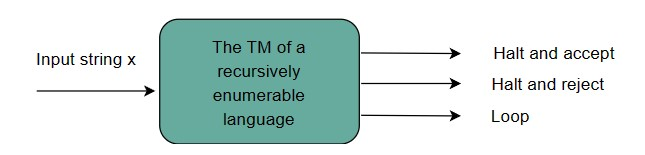
\includegraphics[scale=.65]{img5/m28}
	\caption{The output of a TM running over a recursively enumerable language}
\end{figure}
	\end{itemize}
\end{frame}
\begin{frame}{Recursive and Recursive Enumerable Language}
	\textbf{Recursive Language}
	\begin{itemize}
		\item A language is said to be recursive if there 
		exists a Turing Machine that accepts every string 
		of the language and rejects the string that are 
		not in the language.
		\item A TM of a recursive language never goes into a loop and always halts in every case. Recursive languages are hence also called Turing decidable languages.
		\begin{figure}
			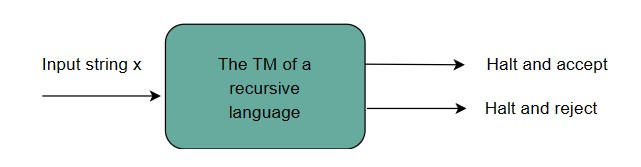
\includegraphics[scale=.65]{img5/m29}
			\caption{The output of a TM running over a recursive language}
		\end{figure}
	\end{itemize}
\end{frame}
\begin{frame}{Recursive and Recursive Enumerable Language}
\begin{itemize}
	\item All the Recursive Languages are
	Recursively Enumerable.
	
	\item Every Recursively Enumerable
	Languages are not Recursive.
	
	\item Recursive Languages are subset
	of Recursively Enumerable
	Languages.
\end{itemize}
		\begin{figure}
			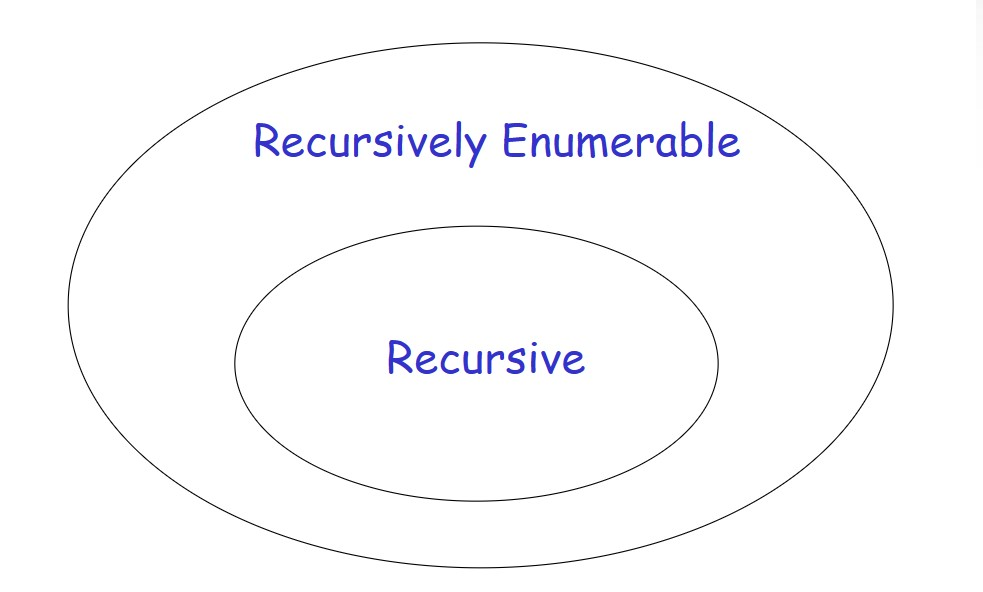
\includegraphics[scale=.4]{img5/m30}
			\caption{Recursive and Recursive Enumerable Language}
		\end{figure}
\end{frame}
\begin{frame}{Recursive and Recursive Enumerable Language}
	\textbf{Closure properties of recursive languages }
	\begin{itemize}
		\item Union
		\item Intersection
		\item Complement
		\item Kleene's closure
	\end{itemize}
\end{frame}

\begin{frame}{Recursive and Recursive Enumerable Language}
	%	\textbf{Closure properties of recursive languages }
	\textbf{Union:}
	\begin{itemize}
		\item The union of two recursive languages $L_1$ and $L_2$ is also a recursive language.
		\item That is, if the TM accepts any one of the languages, it also accepts $L_1\cup L_2$
	\end{itemize}
	\begin{figure}
		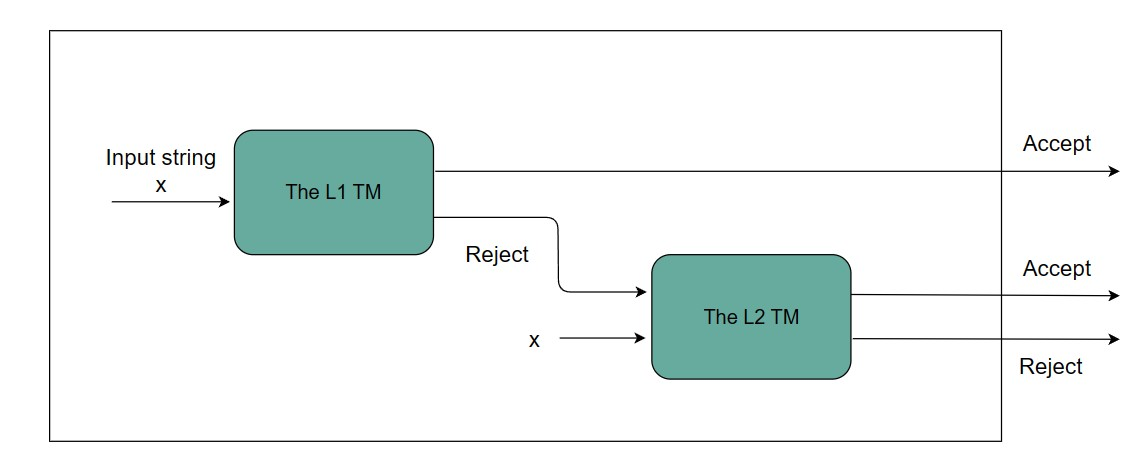
\includegraphics[scale=.4]{img5/m31}
		\caption{The union of two recursive languages}
	\end{figure}
\end{frame}
\begin{frame}{Recursive and Recursive Enumerable Language}
	%	\textbf{Closure properties of recursive languages }
	\textbf{Intersection:}
	\begin{itemize}
		\item  The intersection of two recursive languages $L_1$ and $L_2$ 
		is also a recursive language.
		\item That is, if the TM accepts both languages, it also accepts $L_1\cap L_2$
	\end{itemize}
	\begin{figure}
		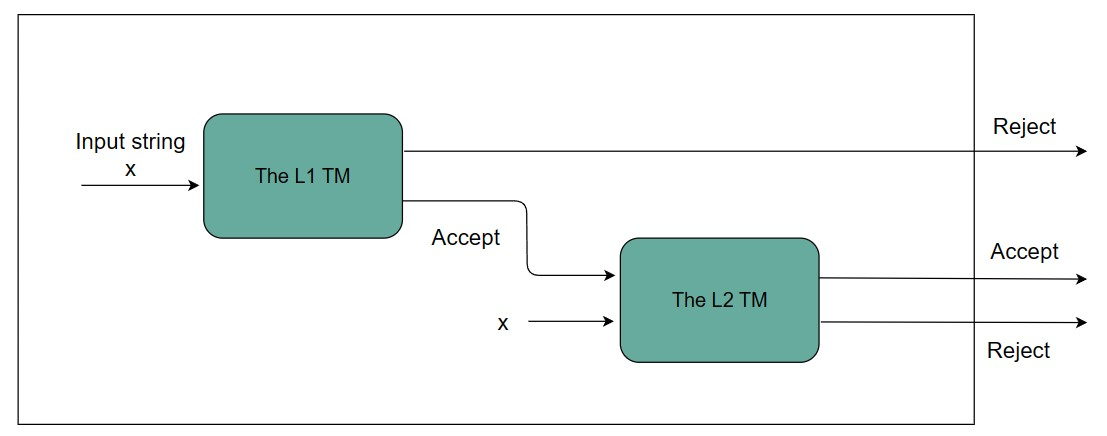
\includegraphics[scale=.4]{img5/m32}
		\caption{The intersection of two recursive languages}
	\end{figure}
\end{frame}
\begin{frame}{Recursive and Recursive Enumerable Language}
	%	\textbf{Closure properties of recursive languages }
	\textbf{Complement:}
	\begin{itemize}
		\item  The complement of a recursive language $L_1$ is also a recursive language. \item That is, if the TM accepts $L_1$ it rejects it as a final output.
	\end{itemize}
	\begin{figure}
		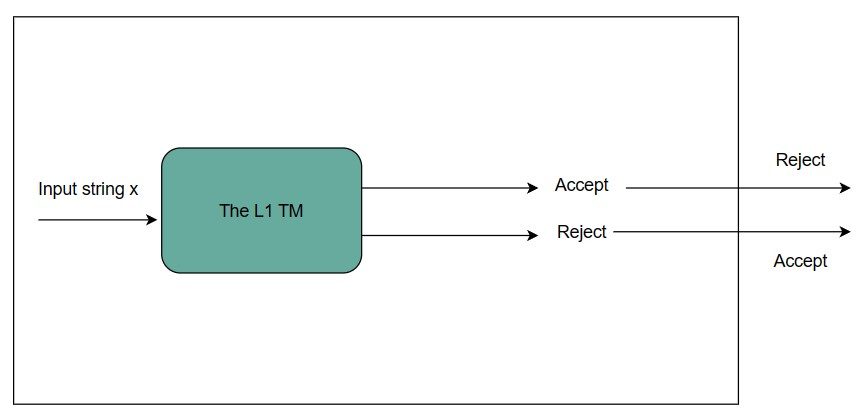
\includegraphics[scale=.4]{img5/m33}
		\caption{The complement of a recursive language}
	\end{figure}

\end{frame}
\begin{frame}{Recursive and Recursive Enumerable Language}
	%	\textbf{Closure properties of recursive languages }
%	\textbf{Complement:}
	\begin{itemize}
		\item If L is recursive, then so is $\bar{L}$.
		\begin{itemize}
			\item LetL be decided by a deterministic M.
			\item Swap the "accept" state and the "reject" state of	M.
			\item The new machine decides	$\bar{L}$
		\end{itemize}
	\end{itemize}
\end{frame}
\begin{frame}{Recursive and Recursive Enumerable Language}
	%	\textbf{Closure properties of recursive languages }
	\textbf{Kleene's closure:}
	\begin{itemize}
		\item The Kleene's closure of a recursive language $L_1$  is also recursive 
		 \item That is, if $L_1=\{o^i1^j\}$ is recursive, then $L_1^*=\{o^i1^j\}^*$  is also recursive.
	\end{itemize}
\end{frame}
\begin{frame}{Recursive and Recursive Enumerable Language}
		\textbf{Closure properties of recursive Enumerable Language } \\
		 Recursive Enumerable Languages are closed under

\begin{itemize}
	\item Union
	\item Intersection
	\item Concatenation
	\item Kleene's closure
\end{itemize}
$^*$ The complement of a recursively enumerable language is not necessarily recursively enumerable. There exist recursively enumerable languages L such that $\bar{L}$(complement of L) is not recursively enumerable.
\end{frame}
\begin{frame}{Recursive and Recursive Enumerable Language}
\textbf{Theorem:} \\
If L is recursively enumerated and $\bar{L}$ is recursively enumerable then L is recursive.
\proofname
\begin{itemize}
	\item Let M and M' be TMs that accept L and $\bar{L}$, respectively. 
	\item Run M and M' simultaneously. 
	\item For any word x, it must be accepted by one of M or M' 
	\item So, either M or M' will halt and accept 
	\item If M halts and accepts then M' halt and reject
	\item If M halts and reject  then M' halt and accepts
\end{itemize}
The TM that runs M and M' simultaneously always halts and accepts or rejects so it decides L 
and L is recursive. 
\end{frame}
\section{Chomsky classification of formal languages}
\begin{frame}{Chomsky classification of formal languages}
		\begin{figure}
		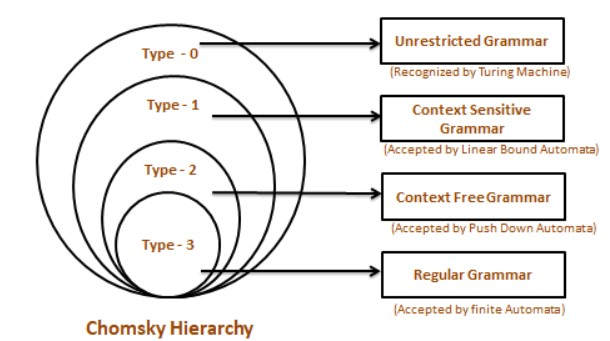
\includegraphics[scale=.8]{img5/m34}
	%	\caption{The complement of a recursive language}
	\end{figure}
\end{frame}
\begin{frame}{Chomsky classification of formal languages}
\textbf{Type 0}
\begin{itemize}
	\item All formal grammars fall under type-0 grammars.
	\item The Turing machine can detect languages with type 0 grammar.
	\item The Recursively Enumerable languages are another name for these languages.
	\item Type 0 Language Production in the form of $\alpha \rightarrow \beta$ where
	\begin{itemize}
		\item $\alpha$ , $\beta$  $\in ( V + T)^*$
		\item V = Variables
		\item T = Terminals.
	\end{itemize}
\item 	In type 0 there must be at least one variable on the Left side of production.
\item For example: 
\begin{eqnarray*}
	S \rightarrow ACaB \\
	Bc \rightarrow acB \\
	CB \rightarrow DB \\
	aD \rightarrow Db
\end{eqnarray*}
\end{itemize}

\end{frame}
\begin{frame}{Chomsky classification of formal languages}
	\textbf{Type 1}
	\begin{itemize}
		\item It is also known as Context Sensitive Language.
		 \item It is recognized by the Linear Bound Automata.
		 \item According to the following rules, context-sensitive grammar:
		 \begin{itemize}
		 	\item It should be Type 0
		 	\item Multiple symbols may be present on the left side of the production rules for the context-sensitive grammar.
		 	\item The number of symbols on the left side cannot be more than the number of symbols on the right side.
		  %\item It does not occur on the right-hand side of any rule.
		 	\item In type 1, Production is in the form of $\alpha A \beta \rightarrow \alpha \gamma \beta$ where $A$ in V, $\alpha$, $\beta \in (V\cup T)^*$and $\gamma \in  (V \cup T)^+$
		 	\item The rule of the form $A \rightarrow \epsilon$ is not allowed unless A is a start symbol.
		 \end{itemize}
	 \item For Example:
	 \begin{eqnarray*}
	 	S \rightarrow AB \\
	 	AB \rightarrow abc \\
	 	B \rightarrow b
	 \end{eqnarray*}
	\end{itemize}
	
\end{frame}
\begin{frame}{Chomsky classification of formal languages}
	\textbf{Type 2}
	\begin{itemize}
		\item It should be Type 1
		\item It is Context-Free Grammar (CFG)
		\item It is recognized by a Pushdown automata
		\item The left-hand side of production can have only one variable and there is no restriction on right side
		\begin{itemize}
			\item  Production is of the form $A \rightarrow \alpha$,
			\item where A is a variable and $\alpha$ is a string of symbols from $(V \cup T)^*$.
		\end{itemize}
		\item For Example:
		\begin{eqnarray*}
		S \rightarrow AB \\
		A \rightarrow a \\
		B \rightarrow b
		\end{eqnarray*}
	\end{itemize}
	
\end{frame}
\begin{frame}{Chomsky classification of formal languages}
	\textbf{Type 3}
	\begin{itemize}
		\item It should be Type 2
		\item It is a Regular Grammar
		\item It can be accepted by a finite-state automaton.
		\item It is the most restricted form of grammar.
		\item It can be described using regular expressions.
		\item These languages can be modelled by NFA or DFA.
		\begin{itemize}
			\item  Production is of the form 
			\begin{eqnarray*}
				V \rightarrow VT / T\  (left- linear\  regular\  grammar) \\
				(or) \\
				V \rightarrow TV /T\  (right - linear\  regular\  grammar)
			\end{eqnarray*}
		\end{itemize}
	 For Example:
	\begin{eqnarray*}
		S \rightarrow aS\\ S \rightarrow bS\\ S \rightarrow a \big | b
	\end{eqnarray*}
	\end{itemize}
	
\end{frame}
\end{document}